\documentclass[tikz]{standalone}
\usepackage{tikz}
\usetikzlibrary{calc,positioning, shapes, petri, automata}
\tikzset{
    transV/.style={transition, fill=black, minimum height = 12mm, minimum width = 1.5mm,inner sep = 0mm},
    transH/.style={transition, fill=black, minimum width = 12mm, minimum height = 1.5mm,inner sep = 0mm},
    node distance=1.5
}
\usepackage{amsmath,amssymb,amsthm,mathrsfs,amsfonts}

\usepackage{csquotes}
\usepackage{booktabs}

\usepackage{graphicx}
\graphicspath{ {../img/} }

\newcommand{\LSset}[2]{\scriptsize $\begin{aligned}&\{#1\}_L\\&\{#2\}_S\end{aligned}$}


\begin{document}    
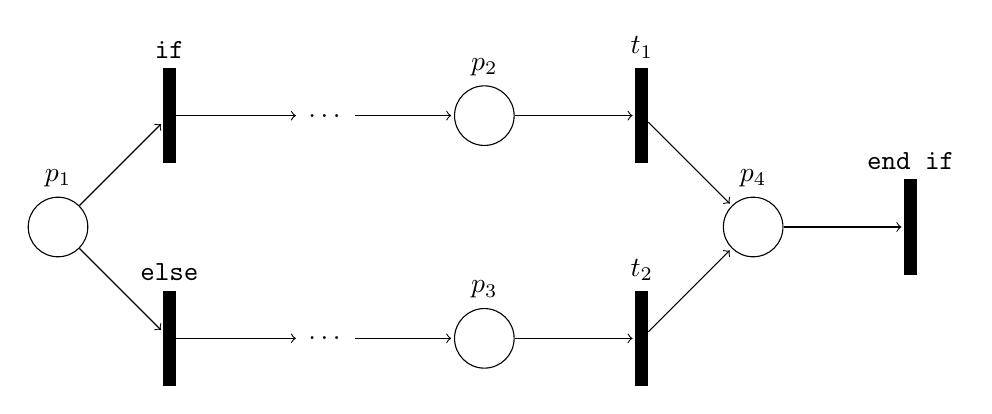
\begin{tikzpicture}[node distance=2cm,on grid, auto]
  \node[place, label=$p_1$] (p1) {};
  \node[transV, label=\texttt{if}, above right = of p1] (if) {};
  \node[transV, label=\texttt{else},below right = of p1] (else) {};
  \node[right = of if] (dots1){$\dots$};
  \node[right = of else] (dots2){$\dots$};
  \node[place, label=$p_2$, right = of dots1] (p2) {};
  \node[place, label=$p_3$, right = of dots2] (p3) {};
  \node[transV, label=$t_1$, right = of p2] (t1) {};
  \node[transV, label=$t_2$, right = of p3] (t2) {};
  \node[place, label=$p_4$, below right = of t1] (p4) {};
  \node[transV, label=\texttt{end if}, right = of p4] (endif) {};



  \draw 
  (p1) edge[post] (if)
  (p1) edge[post] (else)
  (if) edge[post] (dots1)
  (else) edge[post] (dots2)
  (dots1) edge[post] (p2) 
  (dots2) edge[post] (p3) 
  (p2) edge[post] (t1)
  (p3) edge[post] (t2)
  (t1) edge[post] (p4)
  (t2) edge[post] (p4)
  (p4) edge[post] (endif)
  ;
\end{tikzpicture}
\end{document}